\chapter{Evaluation}
\label{cha:eval}
In this chapter, we will evaluate our model with different parameters with the state of art model.
\section{Evaluating different Kernel PCA parameters}
From the figures, \ref{fig:k1} to \ref{fig:k4}, we can determine the appropriate kernel function that can be used for generating Kerneled PCA embeddings. In the figures, \ref{fig:k1} to \ref{fig:k4}, we computed different kernel functions on a set of words and then projected those kernel vectors on a 2-Dimensional space using Kernel PCA.
\begin{figure}[H]
	\begin{minipage}[b]{0.5\linewidth}
		\centering
		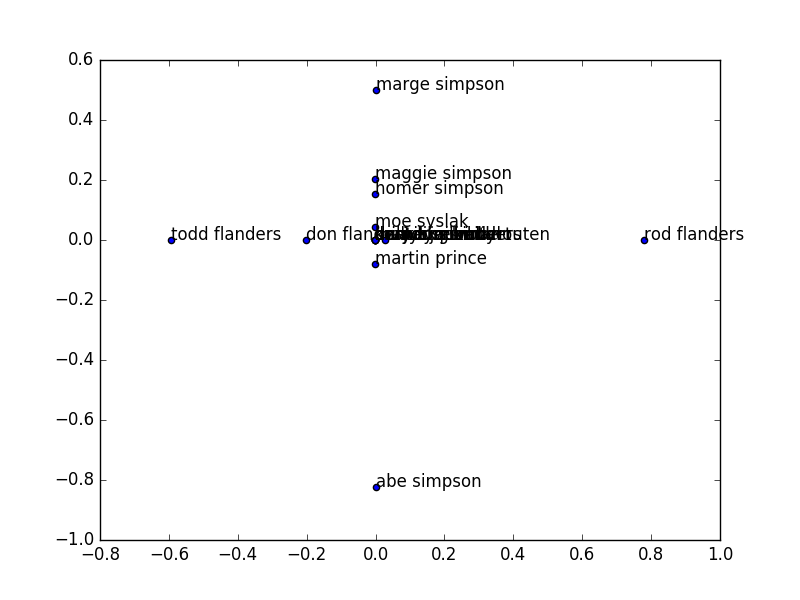
\includegraphics[width=1\linewidth]{files//KERNELPCA/log.png} 
		\caption{Logistic Kernel PCA} 
		\vspace{4ex}\label{fig:k1}
	\end{minipage}%%
	\begin{minipage}[b]{0.5\linewidth}
		\centering
		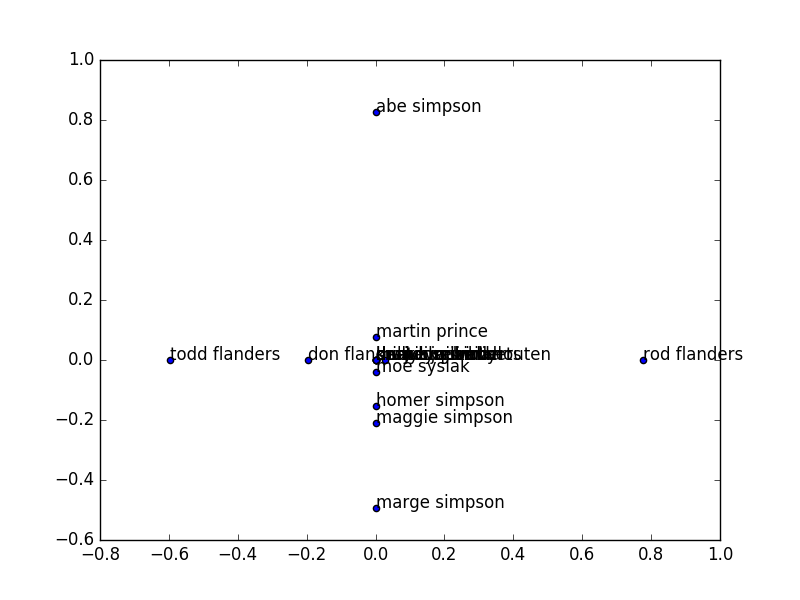
\includegraphics[width=1\linewidth]{files//KERNELPCA/cos.png} 
		\caption{Cosine Kernel PCA} 
		\vspace{4ex}\label{fig:k2}
	\end{minipage} 
\end{figure}
While the logistic and cosine kernel function does not work to cluster similar words together as seen in figures \ref{fig:k1} and \ref{fig:k2}, the polynomial and the Gaussian kernel works best in capturing the morphological similarity of words as demonstrated in figures, \ref{fig:k3} and \ref{fig:k4}. The Gaussian kernel is prominently used in such scenarios because it evaluates the kernel in an infinite dimensional space and hence is very flexible. The parameter sigma of the Gaussian kernel, which represents the co-variance, also plays a major role in its performance as it determine the width of the cluster, and hence should be carefully tuned according to the problem at hand.
\begin{figure}[H]
	\begin{minipage}[b]{0.5\linewidth}
		\centering
		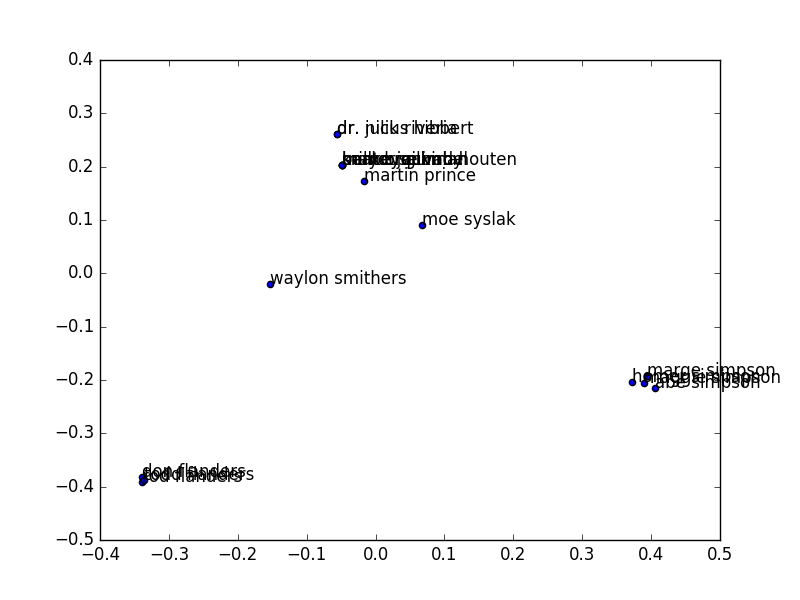
\includegraphics[width=1\linewidth,height=6cm]{files//KERNELPCA/gauss.png} 
		\caption{Gaussian Kernel PCA} 
		\vspace{4ex}\label{fig:k3}
	\end{minipage}%% 
	\begin{minipage}[b]{0.5\linewidth}
		\centering
		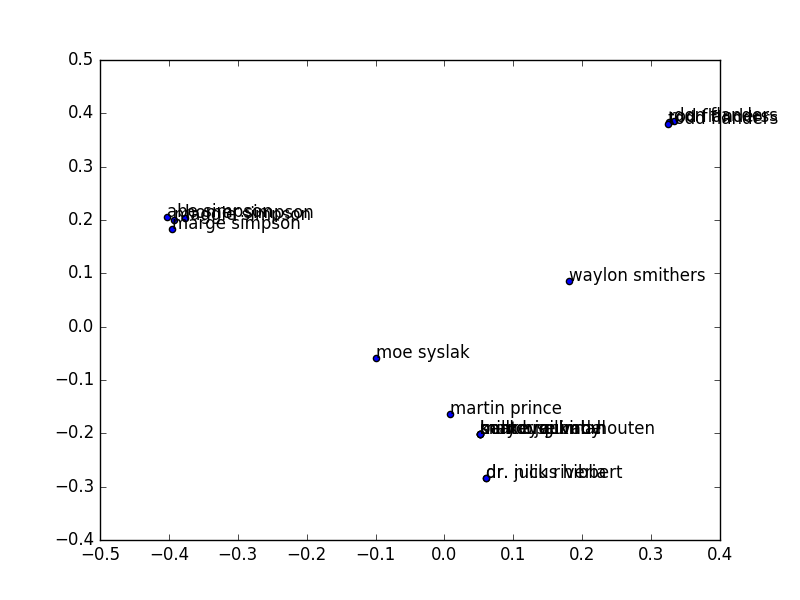
\includegraphics[width=1\linewidth]{files//KERNELPCA/poly.png} 
		\caption{Polynomial Kernel PCA(d=3)} 
		\vspace{4ex}\label{fig:k4}
	\end{minipage} 
	\label{fig:varKernel}
\end{figure}
\section{Evaluating Skip-gram Model trained using KPCA embeddings}
In this section, we will evaluate the performance of our KPCA skip gram model by comparing it against the performance of the basic skip gram model trained on the same parameters. Since the model follows an unsupervised approach, evaluation of the model can only be done using \texttt{"intrinsic evaluation tasks"}, which assess how well the vectors capture the word meaning and the relationships between those words. This is achieved using evaluating the models on the following tasks:
\begin{enumerate}
	\item \texttt{word similarity tasks}, that include finding a word's nearest neighbors.
	\item \texttt{word analogy tasks}, that include calculating the semantic and the syntactic similarity between the words.
\end{enumerate}
The \texttt{pre-trained Google embeddings}, which are considered to be the state of art embeddings, are trained on a dataset of size \texttt{100 Billion} words, with window size \texttt{5}, for \texttt{5} epoch using \texttt{12} threads running in parallel. One major challenge in the skip gram is that we have to train the model on a very large dataset to get the high quality vectors which creates problems, when we don't have a large dataset for training. The disadvantage of training a smaller dataset can  be eliminated by using our approach as we get fairly good quality word vectors, trained on a the relatively smaller dataset like \texttt{Text 8} and \texttt{20News Group} with only \textbf{"one epoch"}. The bad performance of basic skip-gram model in the following results, are  also been attributed to the fact that we are training the vectors on a these dataset. When we train the basic skip gram model on enWiki2016 dataset, as expected, the model starts doing well. 
\subsection{Word similarity Evaluation} 
One approach to evaluate the word embeddings is to see, how well they do in generating \textit{k}-nearest neighbors. This approach helps in visualizing the words and its most related neighbors. In tables \ref{x:1} and \ref{x_:2}, we compared the neighbors of the words, trained on both the models. When analyzed closely we find that our model starts to learn better word vectors rather quickly than the corresponding skip gram model in first few iterations. This is true for both the languages. In \texttt{German}, the results are even better because semantic similarity and morphological similarity converges. Hence fairly good results can be obtained even in fewer steps for morphologically rich languages. 
\begin{table}[H]
	\hskip-0.5cm
	\begin{tabular}[htbp]{|l|l|l|l|}	
		\hline
		\multicolumn{4}{|c|}{\textbf{Comparison between KPCA Skip gram Embeddings and basic Skip gram embeddings}} \\
		\hline
		Step Number&Word &K-PCA Embeddings & Word2vec Embeddings\\ \hline
		\multirow{2}{*}{Step 0} &\textbf{syria:}&syriac, myriad, syrias, myriads & czarist, driver, aurae, revert\\
		&\textbf{christ:}& wrist, purist, christs, wrists &robbing, backups, succeed, feud \\ 
		\hline
		\multirow{2}{*}{Step 20,000} & \textbf{syria:}&syrians, govt, syrian, jordan& czarist, driver, farid, revert \\
		& \textbf{christ:}&lord, christs, depth, messiah & succeed, robbing, axed, somalis \\
		\hline
		\multirow{2}{*}{Step 40,000} &\textbf{syria:}&syrian, jordan, retain, bombard& lebanon, kenneth, charlie, rocco\\
		& \textbf{christ:}&messiah, honor, risen, savior & somalis, succeed, squelch, axed\\
		\hline
		\multirow{2}{*}{Step 80,000} &\textbf{syria:}&syrian, retain, jordan, lebanon& lebanon, font, charlie, rocco\\
		& \textbf{christ:}&christs, savior, atoned, messiah & somalis, squelch, jesus, viscous\\
		\hline
		\multirow{2}{*}{Step 100,000} & \textbf{syria:}&syrian, syrians, jordan, flows& lebanon, font, charlie, rhode\\
		& \textbf{christ:}&christs, messiah, savior, atoned& somalis, squelch, jesus, viscous\\
		\hline
	\end{tabular}
	\caption{The \textit{k}=8-nearest neighbors are generated for vectors of \textbf{300} dimension on a dataset 20NewsGroup of size 17 Million words}\label{x:1}
\end{table}
With increased data set size, our model performed even better for generating the \textit{k}-nearest neighbors since it can learn better relationships by seeing more examples. This can be analyzed from the results in table, \ref{tabb:3}. 
But for the basic skip gram model, the performance is still bad since we are training a relatively smaller dataset with only 1 epoch. We have also demonstrated, in the same table, that our model works fairly well on all categories of words such as verbs, nouns, adjective etc.
\begin{table}[H]
	\hskip-2.0cm
	\begin{tabular}[htbp]{|l|l|l|l|}	
		\hline
		\multicolumn{4}{|c|}{\textbf{Comparison between KPCA Skip gram Embeddings and basic Skip gram embeddings}} \\
		\hline
		Step Number&Word &KPCA Skip gram Model & Skip gram Model\\ \hline
		\multirow{2}{*}{Step 0} &\textbf{macht:}&mitmacht, ohnmacht, aufmacht, ausmacht& witterete, haube, bereisen, skandle\\
		&\textbf{kinder:}&kinder-, rinder, inder, minder &chang,pflaume, schul-\\ 
		\hline
		\multirow{2}{*}{Step 20,000} & \textbf{macht:}&aufmacht, achtung, gelacht, ansinnen&zuercher, malte, naumburg, peitsche \\
		& \textbf{kinder:}&eltern, familien, nachts, festtage& hindurch, bedauert, jahrem winfried \\
		\hline
		\multirow{2}{*}{Step 40,000} &\textbf{macht:}&lacht, vielmehr, mache, anmelden& schon, zuercher, wurde, malte\\
		& \textbf{kinder:}&kindern, eltern, familien, lernen& jahre, schinm wurde, jahren\\
		\hline
		\multirow{2}{*}{Step 80,000} &\textbf{macht:}&machte, mache, sorge, gemacht& schon, immer, meuessen, jahren\\
		& \textbf{kinder:}&kindern, schueler, gruppen, lehrer& schon, jahre, jahren, immer\\
		\hline
		\multirow{2}{*}{Step 100,000} & \textbf{macht:}&mache, machte, gemacht, hoert& schon, immer, muessen, dabei \\
		& \textbf{kinder:}&kindern, gruppen, schueler, freunde& jahren, schon, viele, dabei \\
		\hline
	\end{tabular}
	\caption{The \textit{k}=8-nearest neighbors for vectors of \textbf{300} dimension generated from training the models on the subset of the dataset, \textbf{news.2013.de} of size 52 Million words for the morphological rich language: \textbf{German}} \label{x_:2}
\end{table}
\begin{table}
	\hskip-0.5cm
	\begin{tabular}[htbp]{|l|l|l|l|}	
		\hline
		\multicolumn{4}{|c|}{\textbf{Comparison between KPCA Skip gram Embeddings and basic Skip gram embeddings}} \\
		\hline
		Step No.&Word&K-PCA Embeddings& Word2vec Embeddings\\ \hline
		\multirow{6}{*}{Step 0}
		&\textbf{syria:}& syriac, myriad, syrias, syrian&inland, gally, shoham, myopic\\
		&\textbf{life:}& lmlife, lifes, wife, lift&dergisi, ream, alias, fifth\\
		&\textbf{india:}& indias, indigo2, indict, individ&wish, reuter, quills, ganja\\
		&\textbf{christ:}& wrist, purist, christs, wrists&july, citys, bushes, godism\\
		&\textbf{read:}& 5read, alread, ready, already&divided, masonry, haifa, capsule\\
		&\textbf{israeli:}& elihu, elijah, eliza, elize&rusty, spina, murphys, unites\\ 
		\hline
		\multirow{6}{*}{Step 20,000}
		&\textbf{syria:}& career, birth, your, beer&five, inland, four, zero\\
		&\textbf{life:}& reign, useful, atrophy, images&akita, alias, adder, nine\\
		&\textbf{india:}& induce, lady, vietnam, indulge&wish, three, from, nine\\
		&\textbf{christ:}& osiris, adopts, lips, phobia&july, with, univ, bushes\\
		&\textbf{read:}& survive, proven, involve, task&divided, masonry, haifa, capsule\\
		&\textbf{israeli:}& sylvia, jewry, paolo, elijah&rusty, akita, kansas, above\\ 
		\hline
		\multirow{6}{*}{Step 40,000} 
		&\textbf{syria:}& punjab, ciudad, sinai, libya&inland, five, four, whistle\\
		&\textbf{life:}& stages, career, spirit, faith&akita, zero, alias, adder\\
		&\textbf{india:}& vietnam, iran, berlin, mexico&wish, three, empires, colony\\
		&\textbf{christ:}& lord, jesus, saints, birth&july, bushes, escapes, rabies\\
		&\textbf{read:}& check, respond, tell, wait&divided, masonry, haifa, capsule\\
		&\textbf{israeli:}& serbian, wildly, tribal, weights&rusty, akita, kansas, above\\
		\hline
		\multirow{6}{*}{Step 80,000} 
		&\textbf{syria:}& lebanon, serbia, annexed, latvia&inland, whistle, peddle, judaic\\
		&\textbf{life:}& career, lives, stages, morning&akita, zero, adder, herod\\
		&\textbf{india}:& asian, baltic, brazil, vietnam&canada, africa, five, reuter\\
		&\textbf{christ:}& saints, messiah, prophet, faith&july, lied, citys, escapes\\
		&\textbf{read:}& learn, reader, hear, wants&divided, masonry, haifa, sided\\
		&\textbf{israeli:}& nato, iraqi, defence, inter&rusty, akita, zero, unites\\ 
		\hline
		\multirow{6}{*}{Step 100,000} 
		&\textbf{syria:}& persia, invaded, turkey, ukraine&inland, four, whistle, peddle\\
		&\textbf{life:}& lives, lifes, stages, shadow&akita, adder, zero, herod\\
		&\textbf{india:}& kuwait, vietnam, persia, turkey&thurs, canada, akita, seven\\
		&\textbf{christ:}& saints, messiah, prophet, baptism&july, lied, citys, bushes\\
		&\textbf{read:}& hear, check, learn, reader&haifa, divided, masonry, five\\
		&\textbf{israeli:}& iraqi, syrian, nato, libyan&rusty, akita, federal, murphys\\
		\hline
	\end{tabular}
	\caption{The \textit{k}=8-nearest neighbors are generated for vectors of 300 dimension on a dataset size of \textbf{17 million words}}\label{tabb:3}
\end{table}

We can also visualize, how well our model did by plotting the t-SNE embeddings of a subset of words from the dictionary.
In this evaluation, we have used \texttt{t-SNE} to project word embeddings on a 2 dimensional space to get a better visualization of the similar word vectors. We obtained visualization of these t-SNE plots for embeddings trained on different datasets and vocabulary sizes, plotted in figures \ref{fig:tsnee1} to \ref{fig:tsnee5}. As expected, we can see that the words which have high similarity are clustered. On comparing t-SNE of our approach with that of skip gram model, we can very easily say that similar words clusters are more prominent in our approach. 

On further analysis of these plots, we can say that even when we add more words to our small vocabulary fig. \ref{fig:tsnee3}, its performance is very much comparable to the fig. \ref{fig:tsnee2}. This proves that we can increase our vocabulary easily with \textbf{Out-Of-Vocabulary words} using method explained in the section \ref{oov}, before training the skip gram model with KPCA embeddings. We also analyzed that there is not a prominent drop in performance of our model when a large number of words are added. It still performs better than the corresponding skip-gram model as seen in figure, \ref{fig:tsnee1}. \\
We also saw the effect of data set size on the basic skip gram performance in figures, \ref{fig:tsnee1} and \ref{fig:tsnee5}. After analyzing these t-SNE plots, we can confidently say that the skip gram model's performance for clustering the similar words starts improving, when it is trained on a bigger dataset. In figure, \ref{fig:tsnee5}, since the dataset is of size 52 million words, we can trace some clusters.
\begin{figure}[H]
	\hskip-2cm
	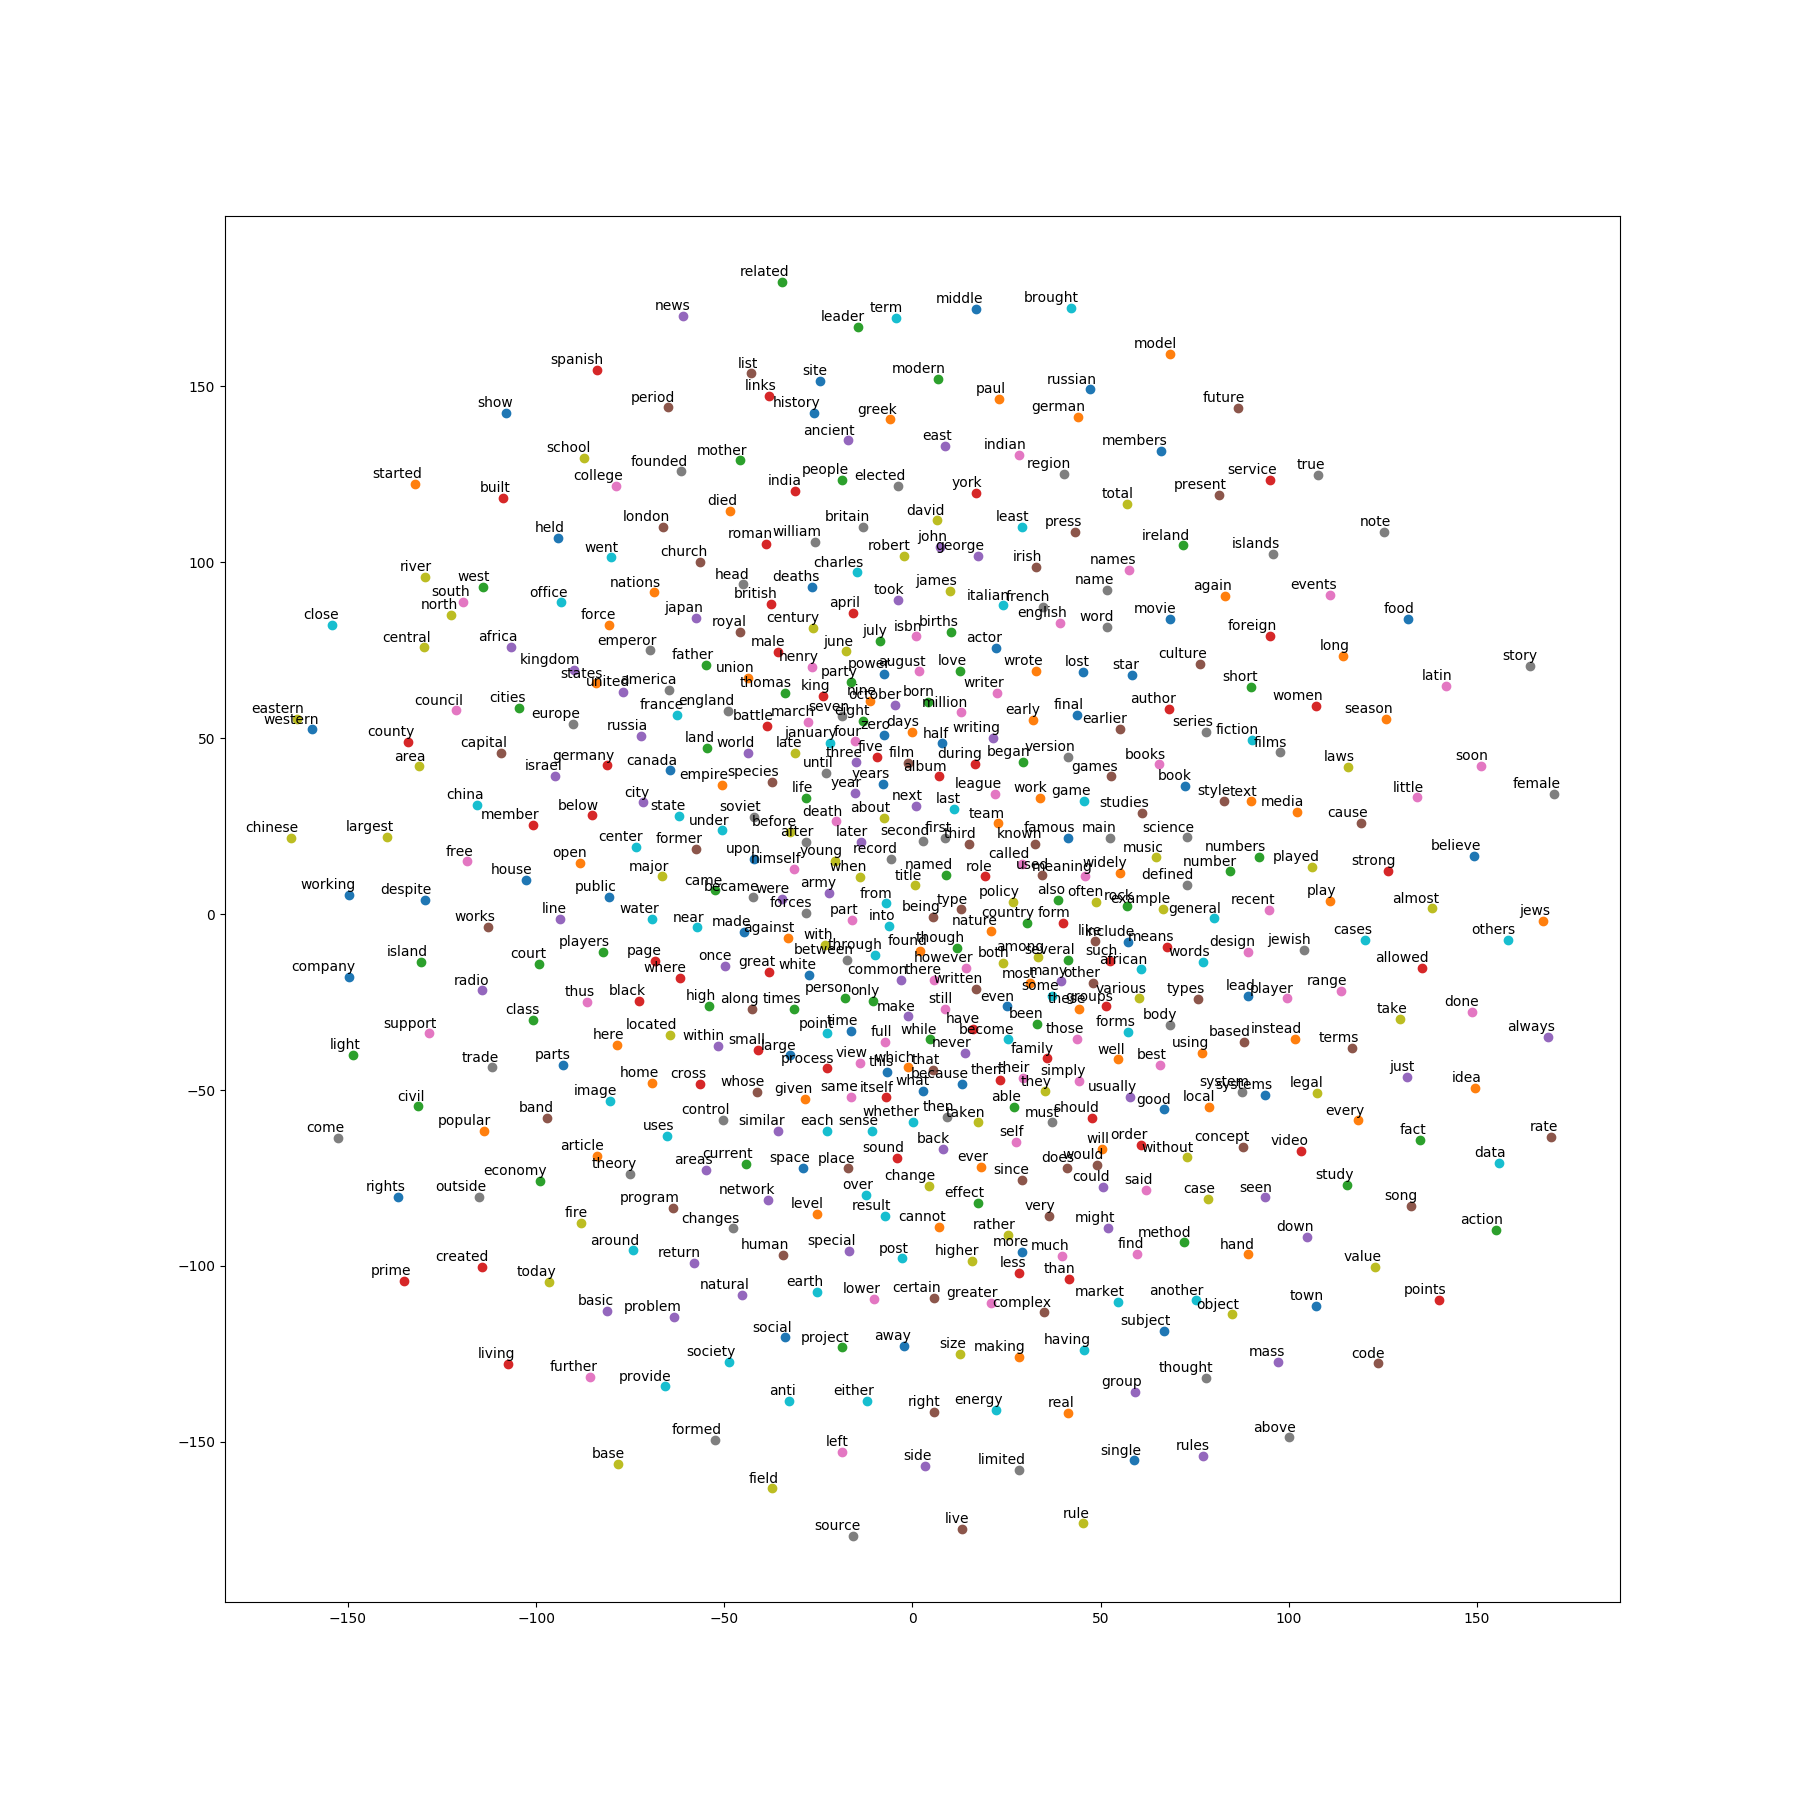
\includegraphics[width=20cm,height=20cm,keepaspectratio]{files/enText8-20kExtendedVocab/w2vtsne.png}
	\caption{t-SNE visualization of Skip gram model with vocabulary size 118,000 trained in 100,000 iteration on Text8 dataset. On analyzing this plot, we cannot find any prominent cluster. The bad performance of the model can be attributed to the fact that we are training the model on a relatively smaller database for 1 Epoch. The performance ought to improve when we train the model for more epoch which is illustrated in later section, in table,\ref{tab:sesx}}
	\label{fig:tsnee1}
\end{figure}
\begin{figure}[H]
	\hskip-2cm
	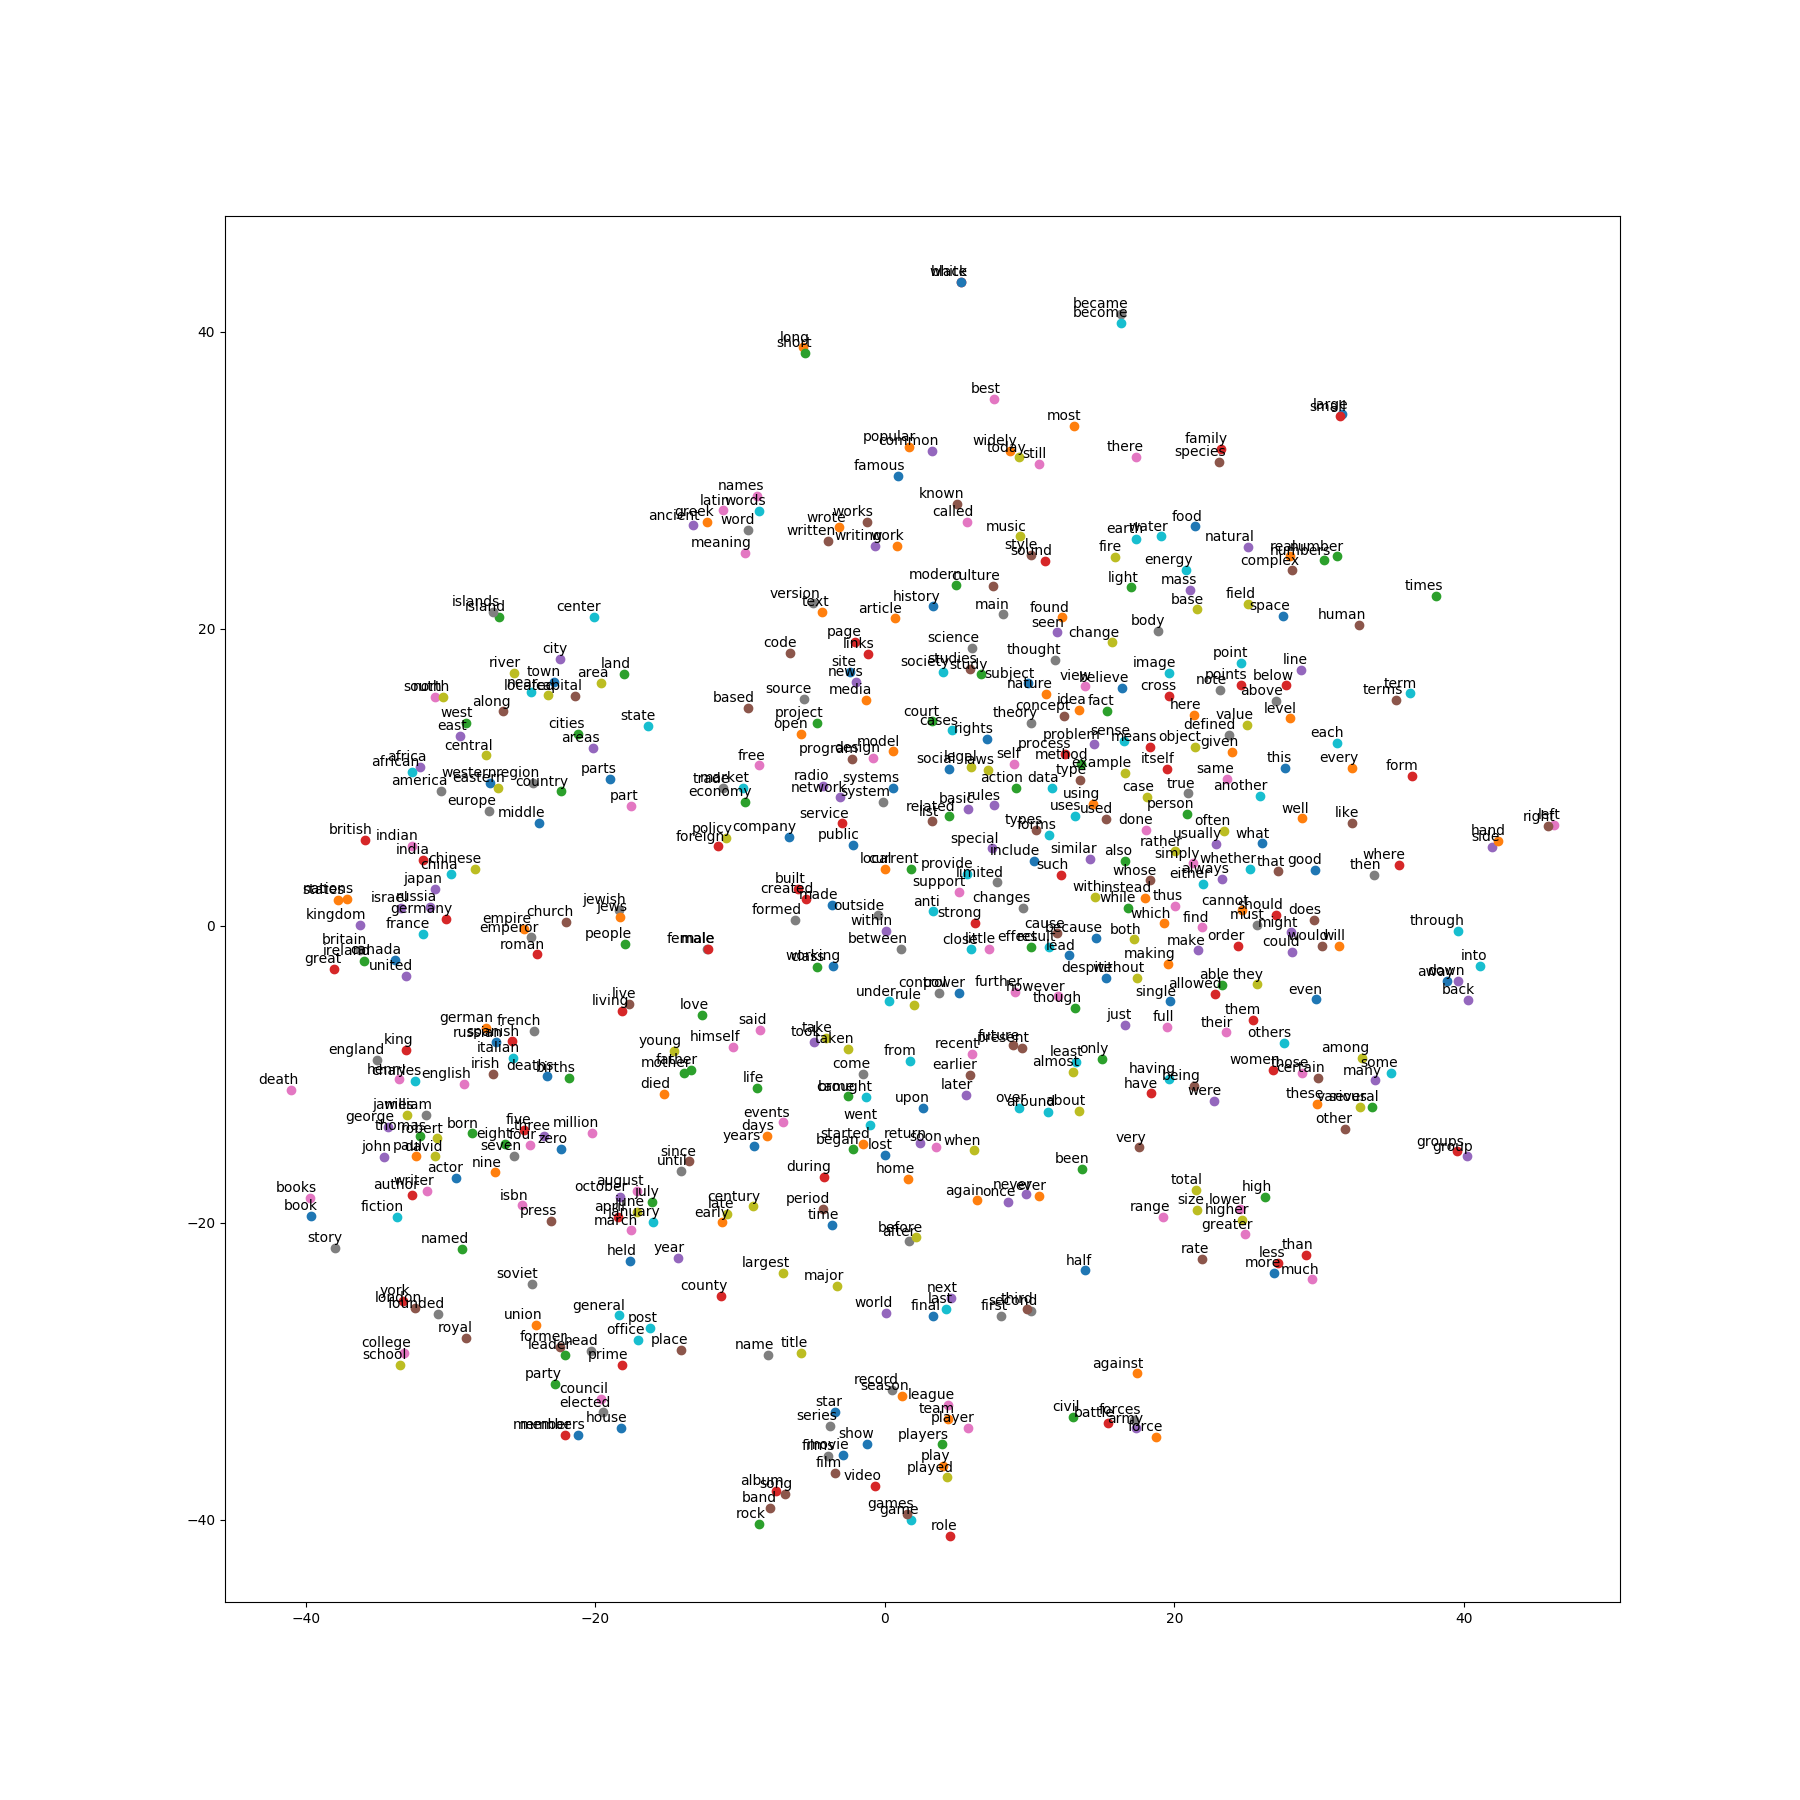
\includegraphics[width=20cm,height=20cm,keepaspectratio]{files/enText8-20kExtendedVocab/text8V20000.png}
	\caption{t-SNE visualization of KPCA Skip gram Word embeddings for vocabulary size 20,000, trained in 100,000 iterations on Text8 dataset of size 17 Million words. If analyzed closely, we find all the nations are clustered together. First names, natural areas, hobbies types and degree of comparison also form very prominent clusters.}
	\label{fig:tsnee2}
\end{figure}
\begin{figure}[H]
	\hskip-2cm
	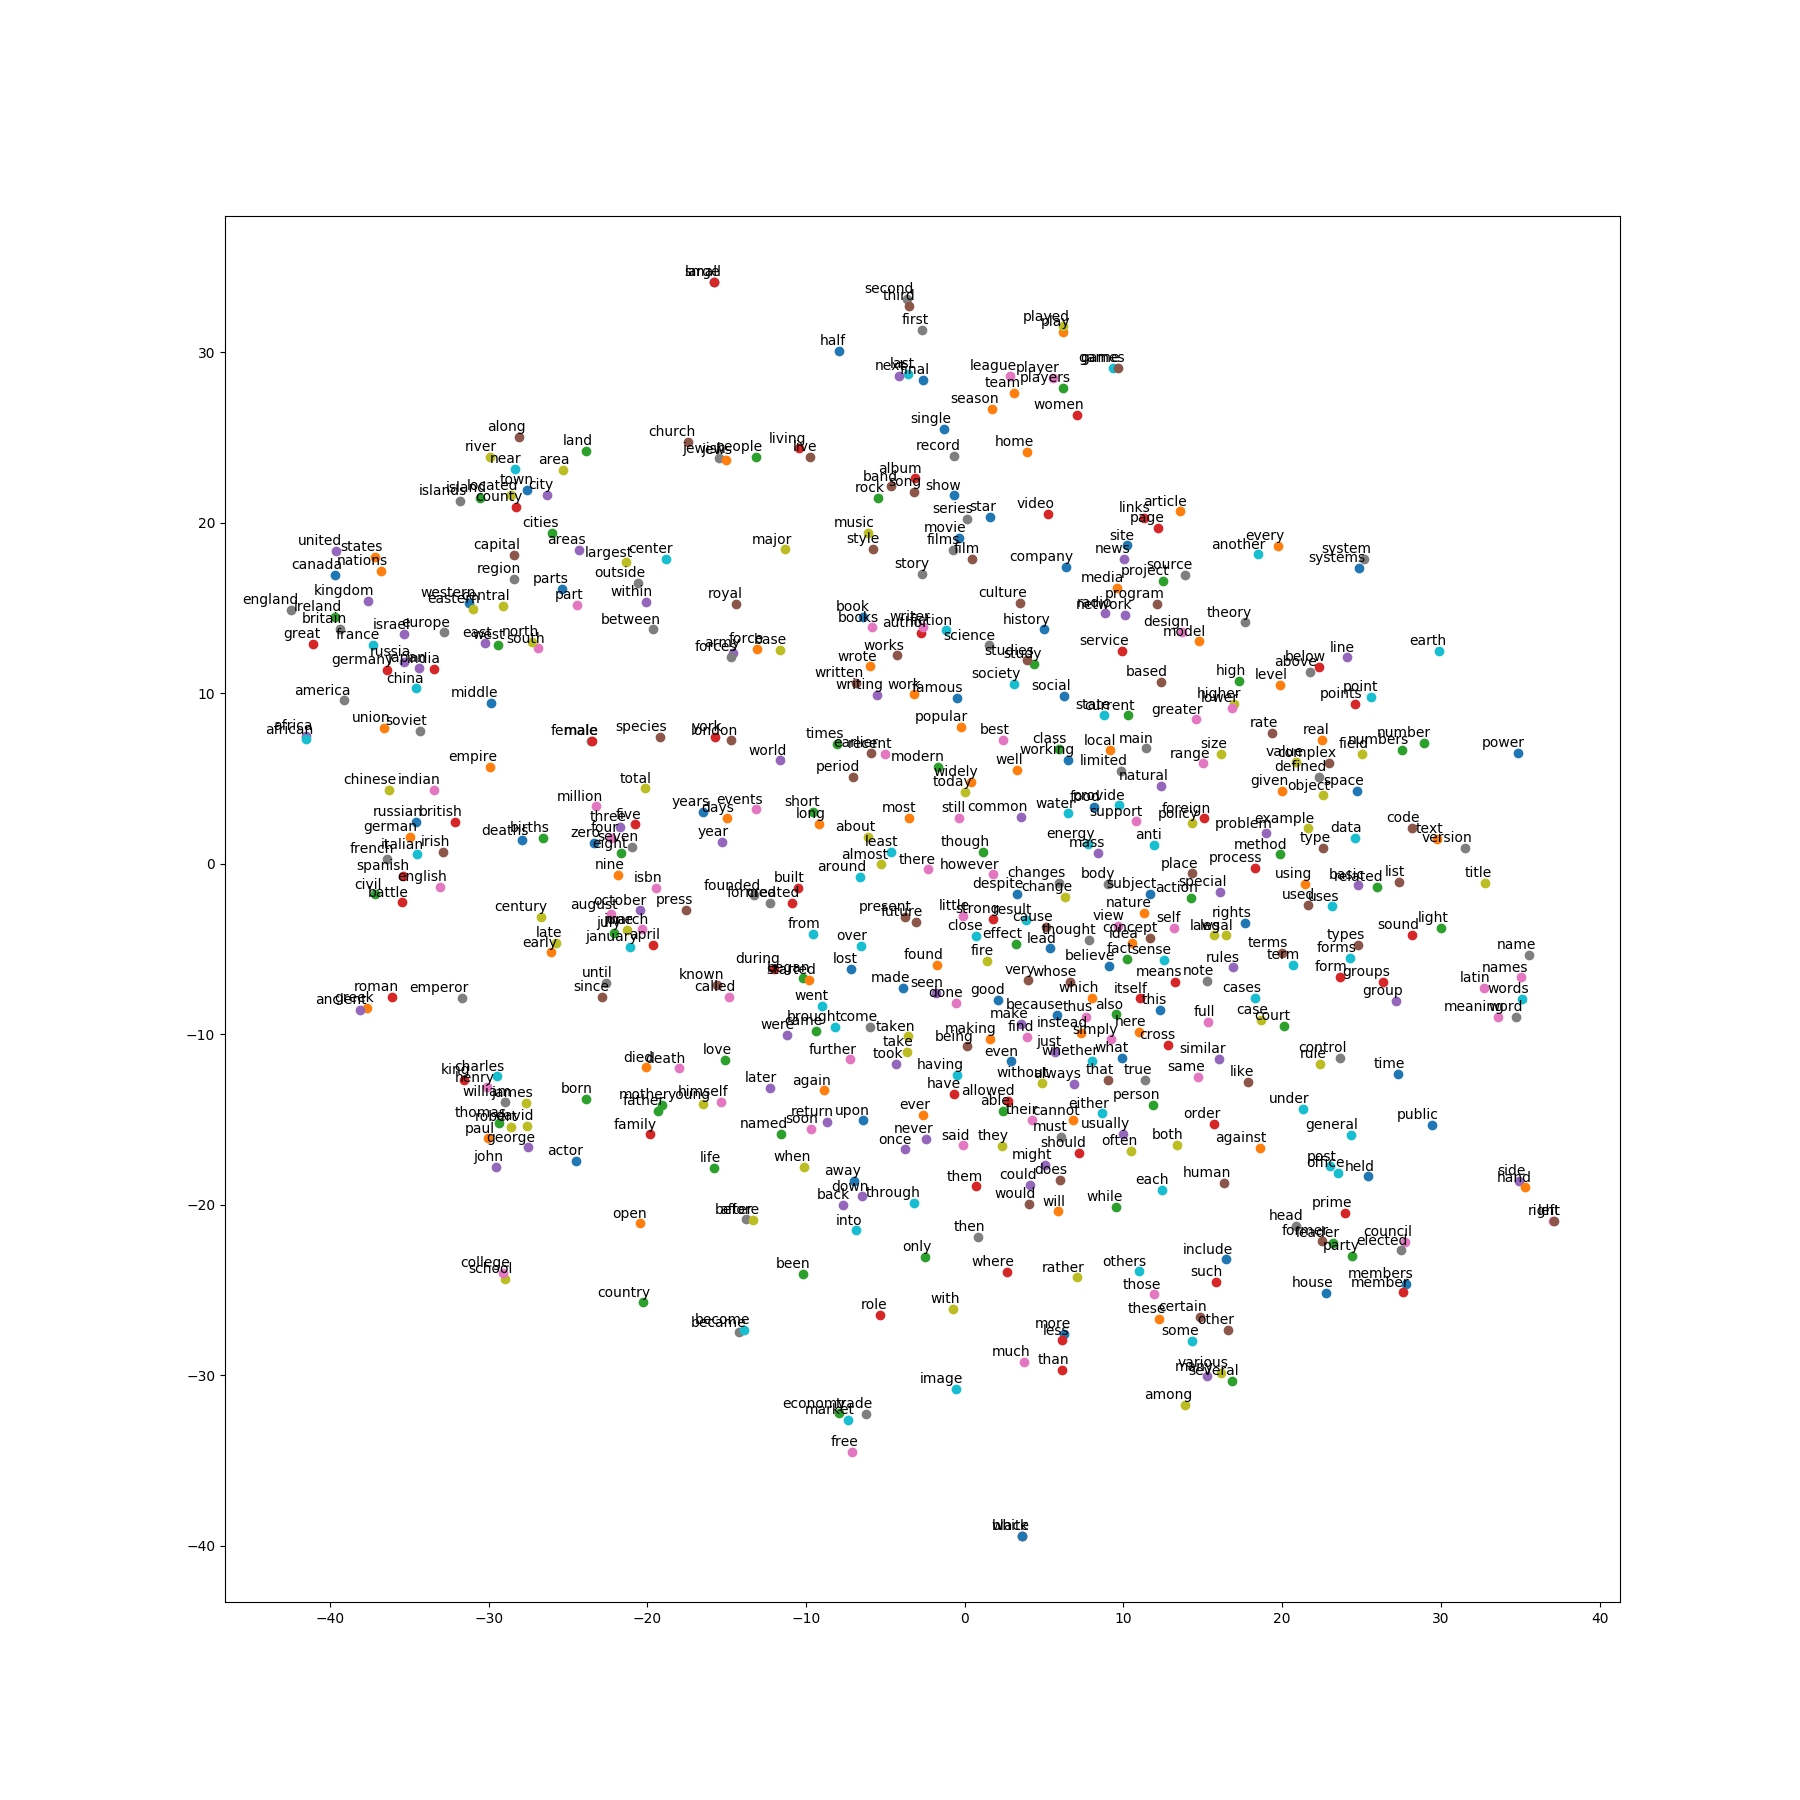
\includegraphics[width=20cm,height=20cm,keepaspectratio]{files/enText8-20kExtendedVocab/tsne.png}
	\caption{t-SNE visualization of KPCA Skip gram embeddings with Vocabulary size 20,000 words extended to 118,000 words, trained in 100,000 iteration on Text8 dataset of size 17 Million words. If analyzed closely, we find clusters of nationality, nations, first names etc. Another important thing to note is that clusters of the nationality and the nations also lie close to each other. }
	\label{fig:tsnee3}
\end{figure}

\begin{figure}[H]
	\hskip-2cm
	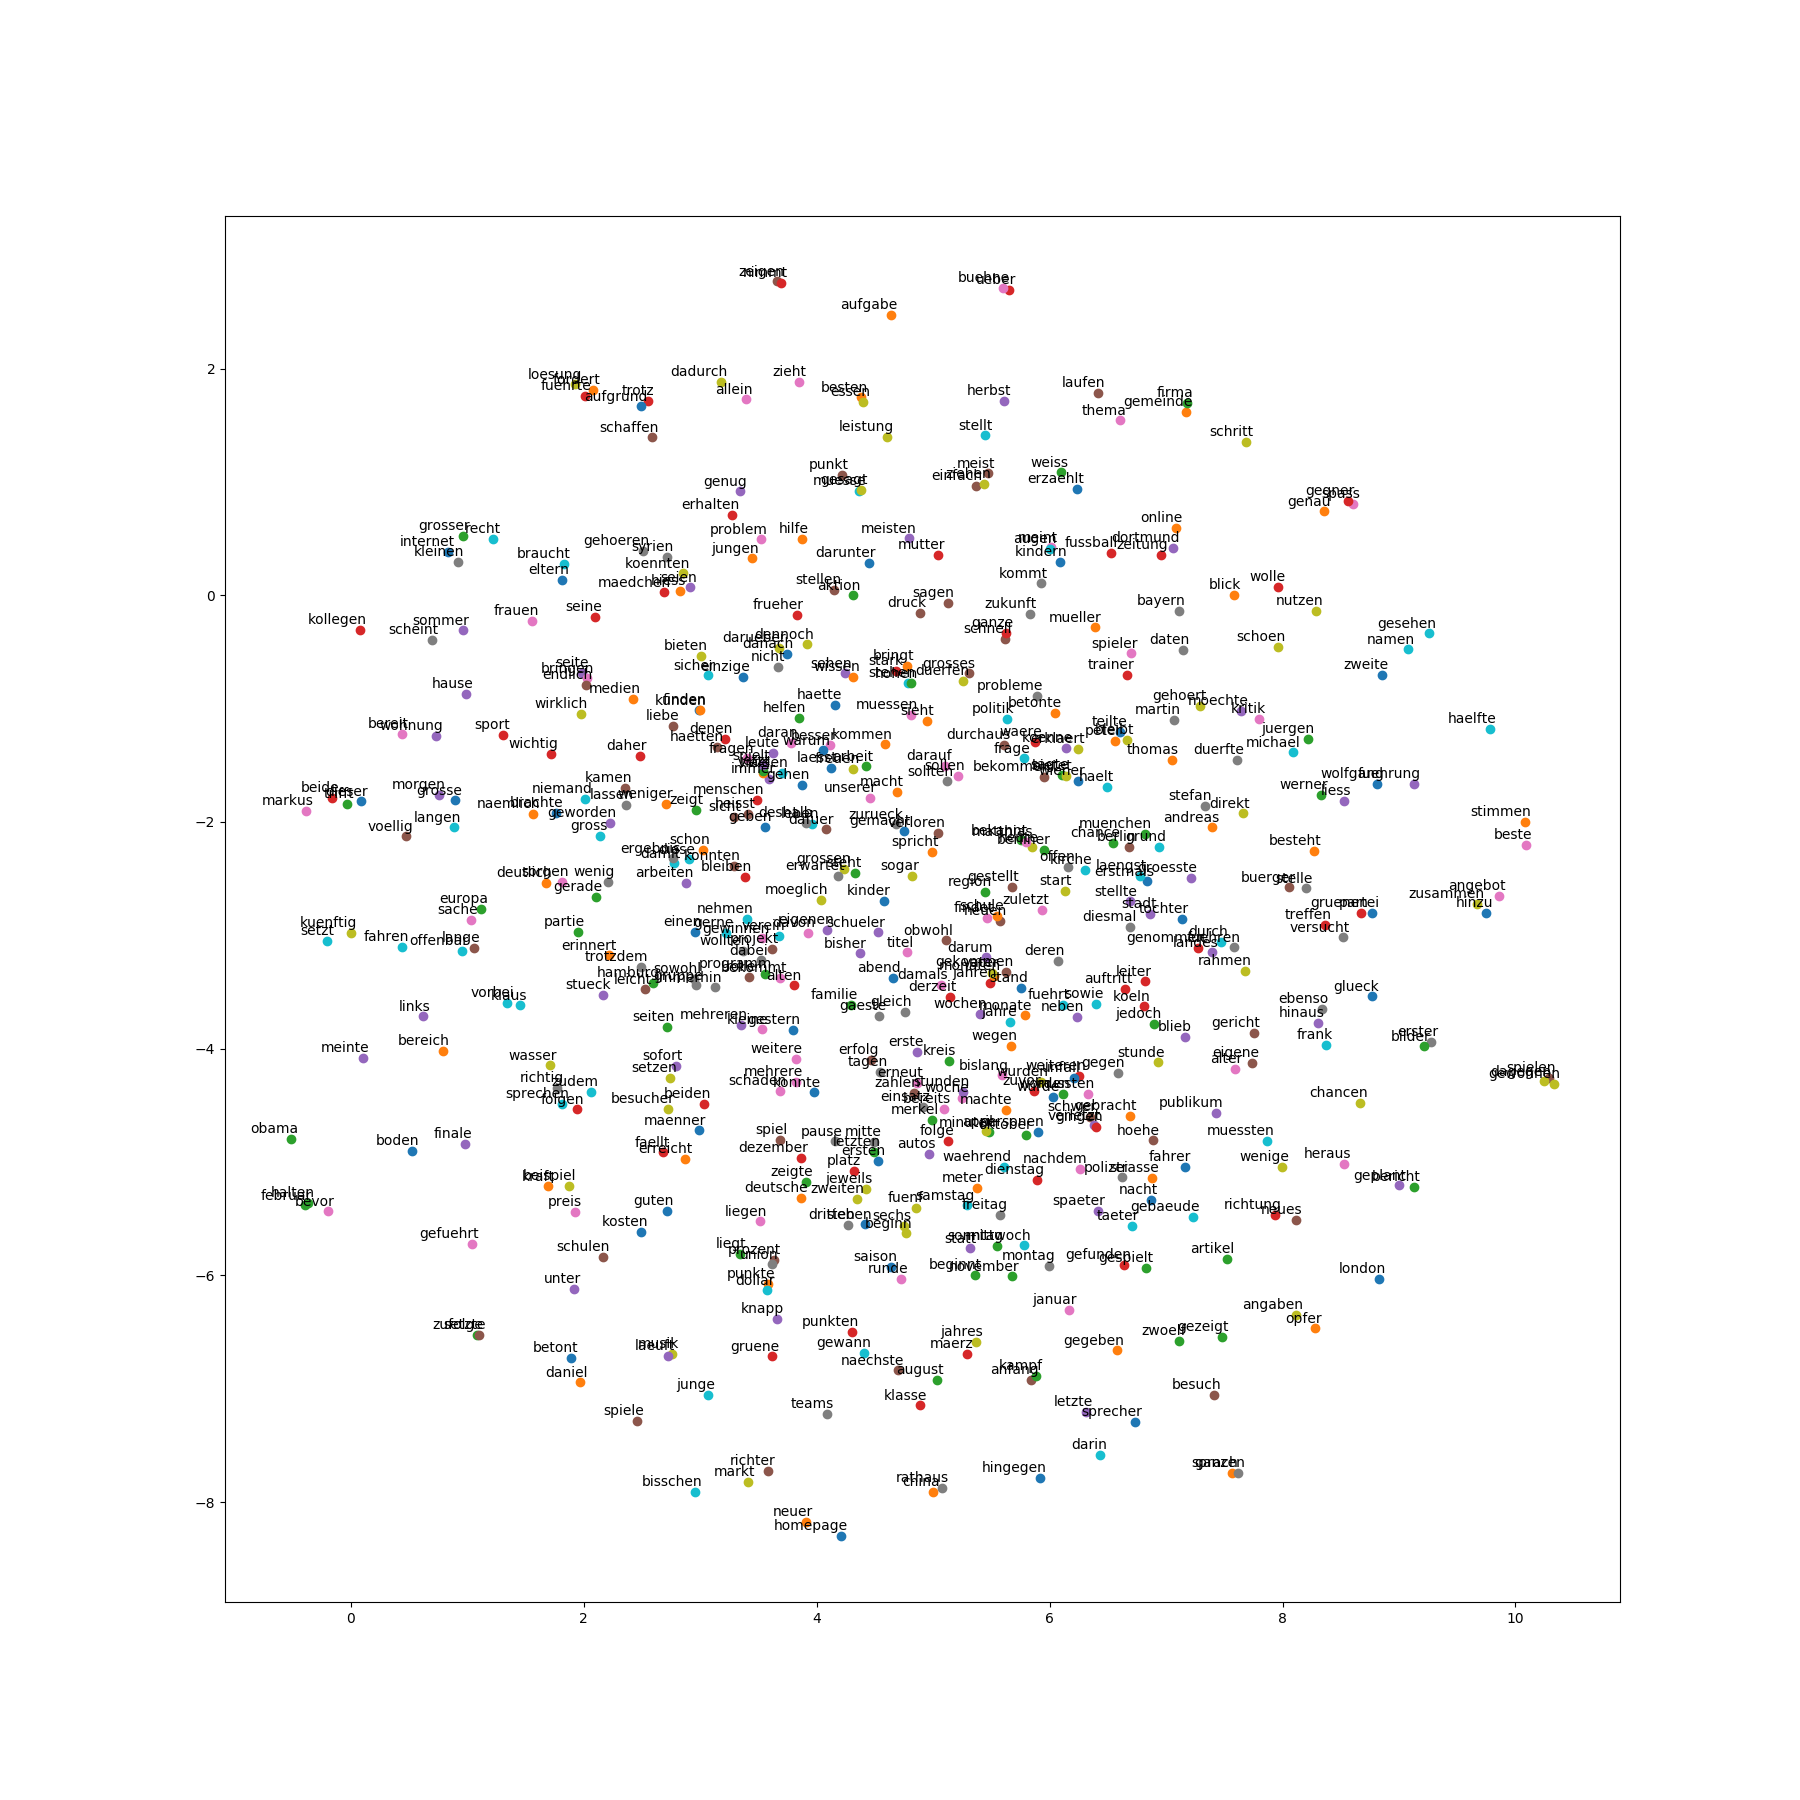
\includegraphics[width=20cm,height=20cm,keepaspectratio]{files/deWiki20kVocab/tsne.png}
	\caption{t-SNE visualization of Skip gram model with Vocabulary size 20,000 trained in 100,000 iteration on a subset of dataset news.2013.de.shuffled.corpus of size 52 Million words. When analyzed closely, we find verbs such as "nehmen", "arbeiten", "bleiben" got clustered together. Other example is words like "mehreren", "mehrere", "weiter" also got clustered}
	\label{fig:tsnee4}
\end{figure}
\begin{figure}[H]
	\hskip-2cm
	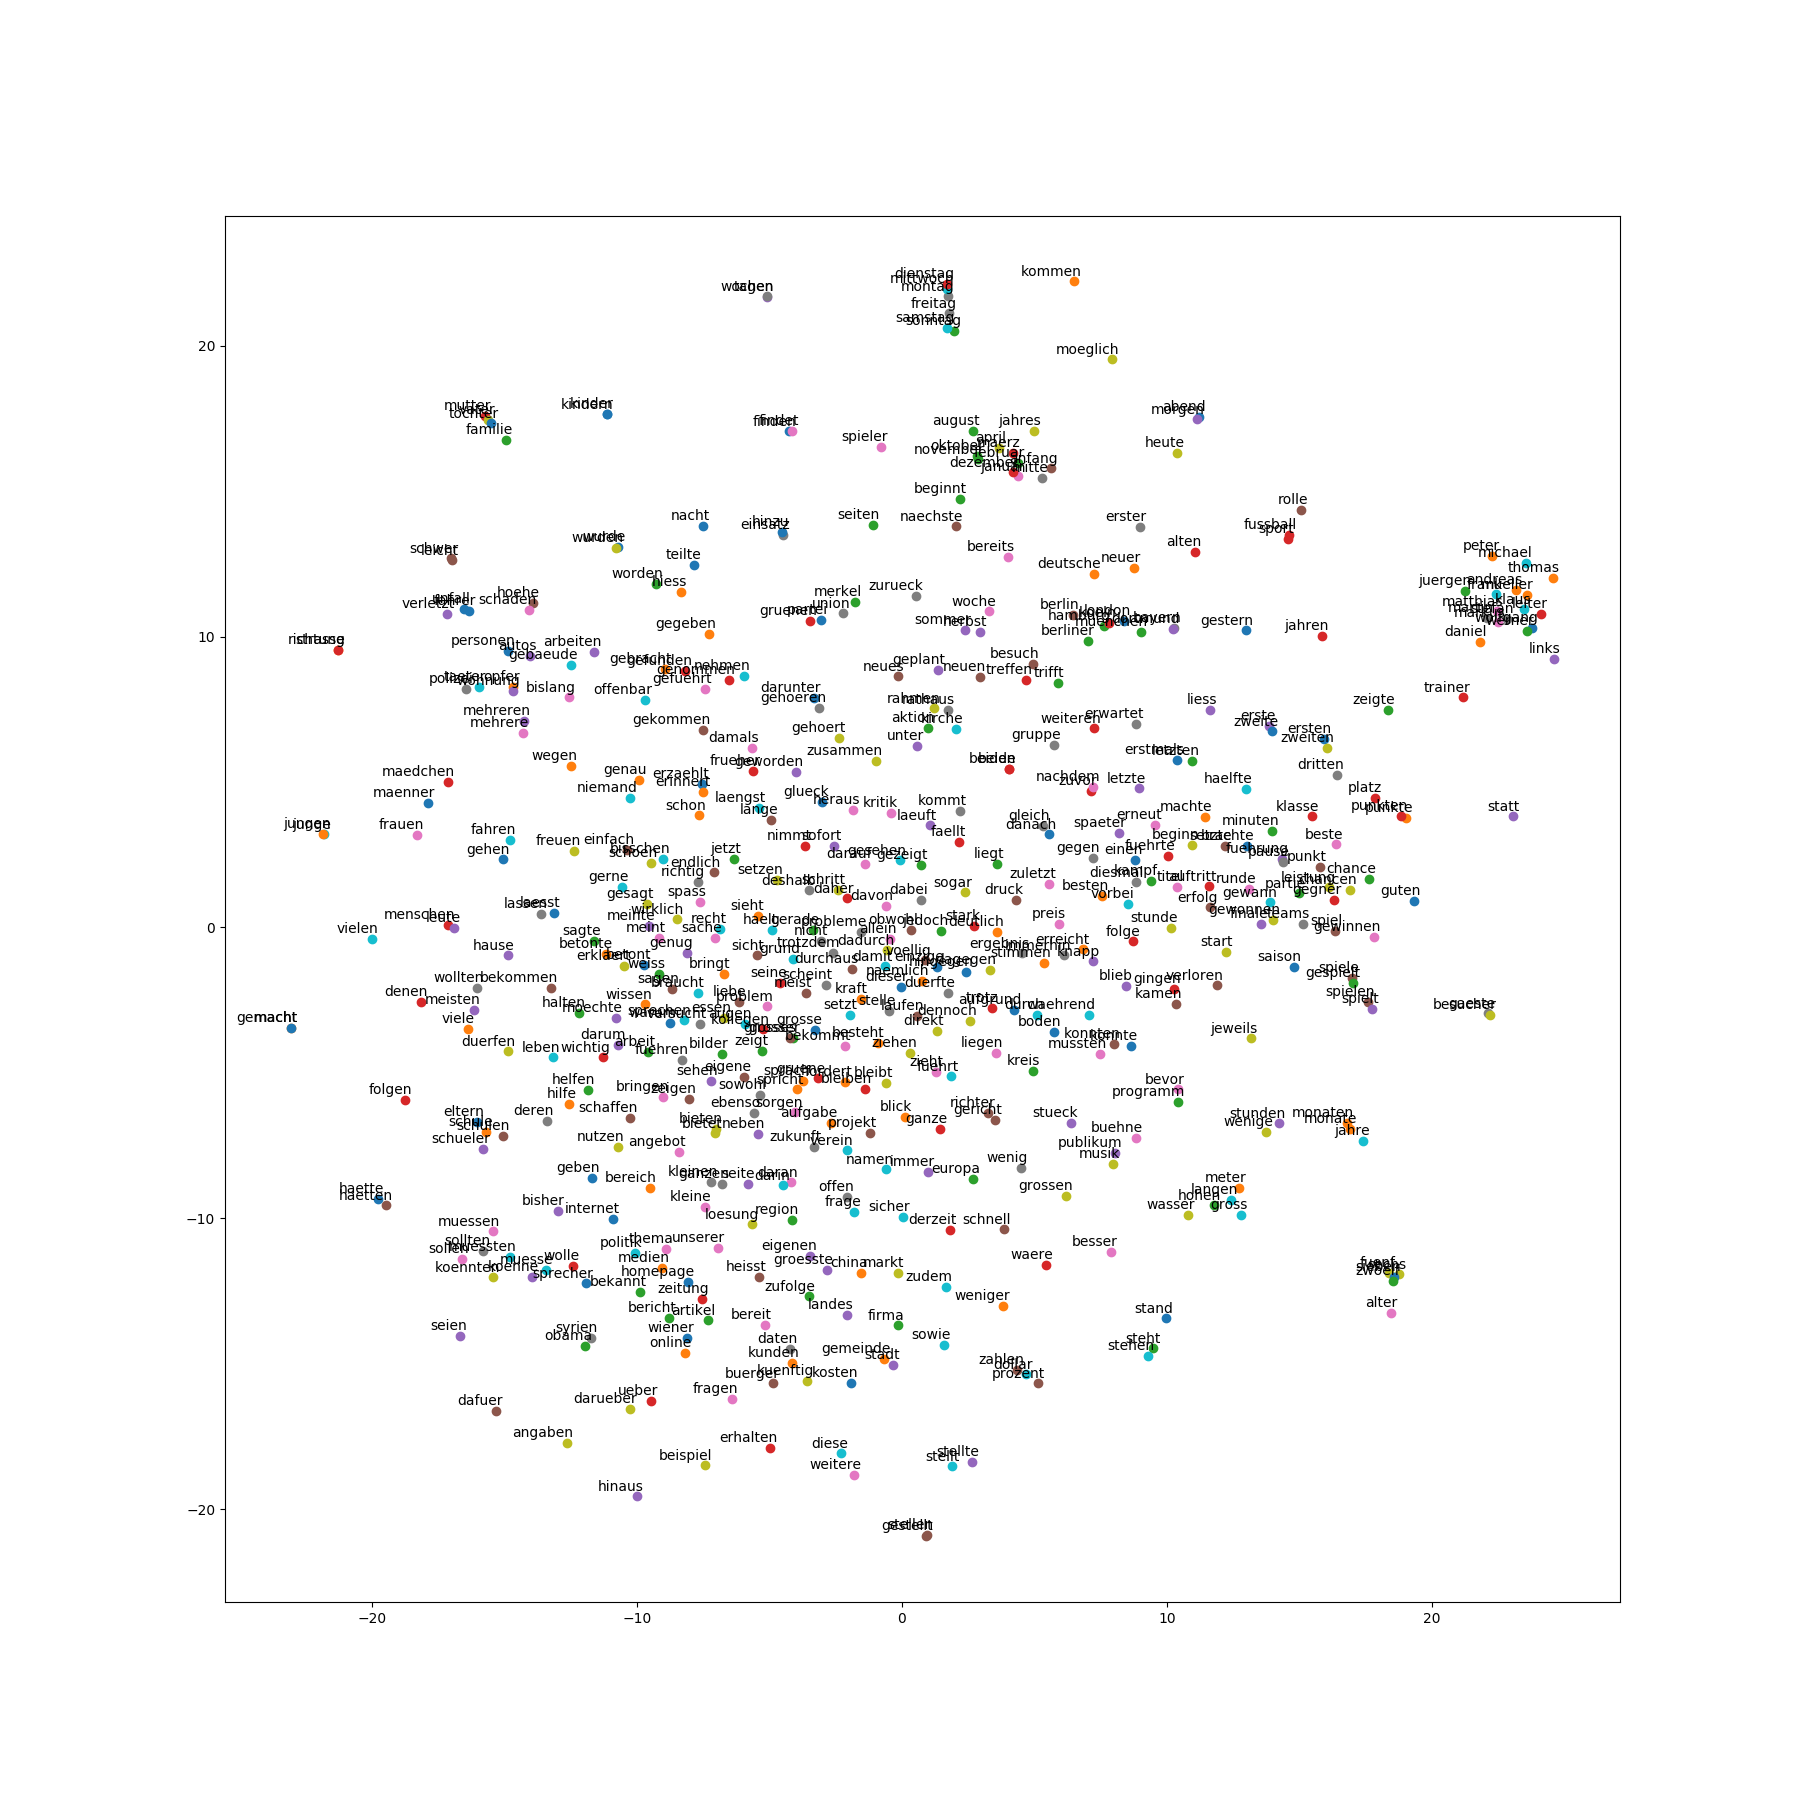
\includegraphics[width=20cm,height=20cm,keepaspectratio]{files/deWiki20kVocab/MYtsne.png}
	\caption{t-SNE visualization of KPCA Skip gram embeddings with vocabulary size 20,000 trained in 100,000 iteration on a subset of dataset news.2013.de.shuffled.corpus of size 52 Million words. When analyzed closely, we find prominent clusters of weekday names, first names, family memeber types etc.}
	\label{fig:tsnee5}
\end{figure}
 
To summarize word similarity evaluation, we can say that KPCA Skip gram Model performs far better than the basic skip gram model. This can be attributed to the fact that we already have trained the vectors for morphological similarities. The model just needs to learn the semantic and syntactic similarity. Since basic skip gram model learns morphological similarity implicitly so initializing the model with those helps in speed up the process of convergence. The performance is even better when the language is rich in morphemes such as German.
%% german k nearest neighbors for 300 dim
\subsection{Word Analogy Evaluation}
In their paper, \cite{mikolov2013efficient} stated that when we train the high dimensional word vectors on a very large data set, the vectors also learn very subtle relation between the words, for example relationships between the country and its capital city.  The figure, \ref{fig:t3}, from paper \cite{mikolov2013distributed}, demonstrates such a relationship. 
\begin{figure}[H]
	\centering
	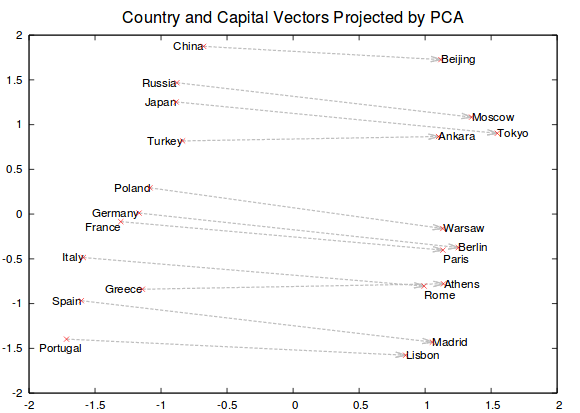
\includegraphics[width=10cm,height=8cm,keepaspectratio]{files/3.png}
	\caption{ Two-dimensional PCA projection of the \textbf{1000-dimensional} Skip-gram vectors of countries and their capital cities as demonstrated by \cite{mikolov2013distributed}}
	\label{fig:t3}
\end{figure}
The data set used to obtain these state of art results, was of 6 Billion words in size and vector dimensions produced were of 1000 dim. In this comparison, our model learned these relationship quickly  we already have morphological similarities encoded in the input vectors. Thus we do not need a large amount of data to train our model. This is very well demonstrated in the figures \ref{fig:t} and \ref{fig:d} where we have plotted the country and the capital relationships for both the models (in both the languages). From these plot we can state that our model has learned these similarity not only in fewer steps but also in a lower dimensional space when compared to the basic skip gram trained using the same parameters. 
\begin{figure}[htbp]
	\centering
	\subfloat[KPCA skip gram model]{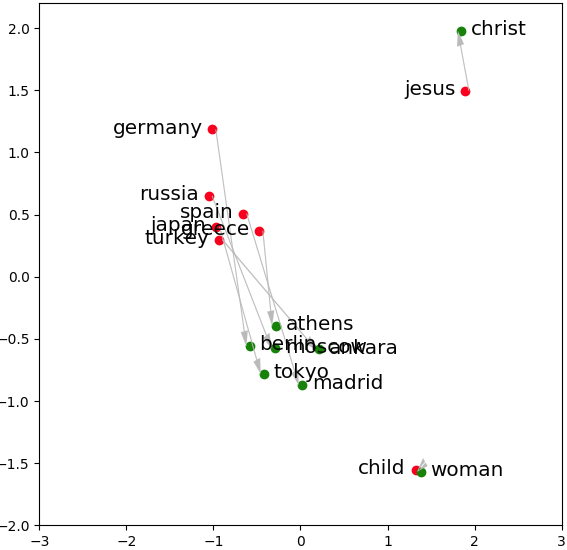
\includegraphics[width=3in,height=3in]{files/2.png}}
	\subfloat[Basic skip gram model]{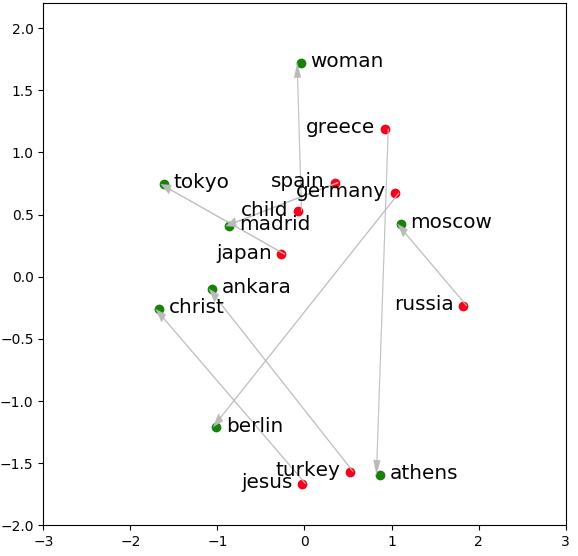
\includegraphics[width=3in,height=3in]{files/1.png}}
	\caption{Two-dimensional PCA projection of the \textbf{300-dimensional} skip gram vectors of countries and their capital cities trained on \textbf{English language} in 100,000 iterations on subset of dataset \texttt{Text8}. Countries(Red labels)and Captials(green labels)}\label{fig:t}
\end{figure}
\begin{figure}[htbp]
	\centering
	\subfloat[KPCA skip gram model]{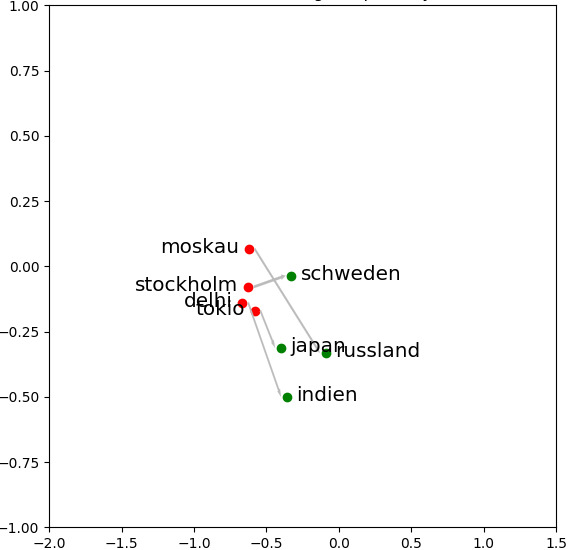
\includegraphics[width=3in,height=3in]{files/de1.png}}
	\subfloat[Basic skip gram model]{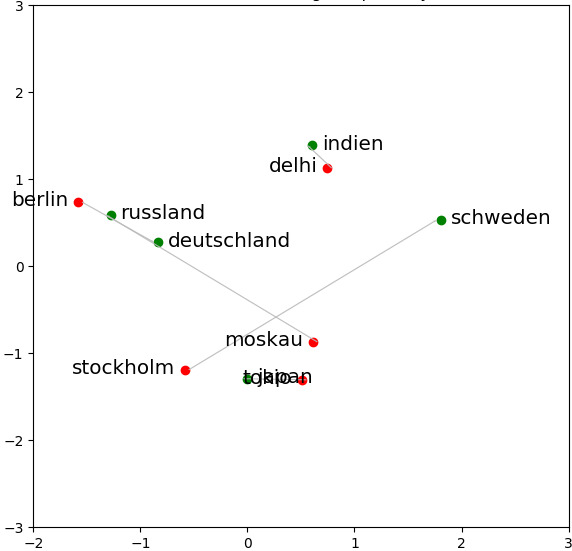
\includegraphics[width=3in,height=3in]{files/de2.png}}
	\caption{Two-dimensional PCA projection of the \textbf{300-dimensional} Skip-gram vectors of countries and their capital cities trained on \textbf{German language} in 100,000 iterations on subset of dataset \texttt{news.2013.de.shuffled.corpus}. Countries(Red labels)and Captials(green labels)}\label{fig:d}
\end{figure}

We have also calculated the accuracy of word analogy task using a \texttt{comprehensive test set}, which has been proposed and used by \cite{mikolov2013efficient} to evaluate their embeddings. The test consists of "semantic" and "syntactic" similarity questions. There are in total $19544$ questions which include relationships like: 
\begin{enumerate}
	\item adjective-to-adverb relationship
	\item capital-world relationship
	\item currency relationship
	\item plural-verbs relationship
	\item city-in-state relationship
	\item comparative relationship
	\item superlative relationship
	\item and many more...
\end{enumerate}
The test set computes the overall accuracy for all question types and is considered correctly answered only if the closest word to the vector computed is exactly the same as the correct word. Thus synonyms are considered as a wrong answer. \cite{mikolov2013efficient} has stated that to get these similarities, we need to train our model on a very large dataset. They have also reported that when they trained their model on a data set of size as big as \texttt{1.6 Billion or 768 Million words}, they obtained state of art accuracy even for \textbf{1 Epoch}.\\

In order to use this evaluation and to compare our model's results with basic skip gram as well as to the state-of-art results, we have trained our KPCA skip gram model and the basic skip gram model, on a smaller data set \textbf{Text8} as well on a huge data set, \textbf{en Wiki 2016}. We have also varied the number of epochs for training the smaller dataset(17 Million words) but only 1 epoch for larger dataset(1 Billion words) as stated by \cite{mikolov2013efficient}. Tests for the accuracies with different dictionary sizes for both the models have also been run.  
The performance of KPCA Skip gram and Basic Skip gram are reported in the tables \ref{ses1}, \ref{ses2} and \ref{tab:sesx}.  
\begin{table}[H]
	\hskip-1.0cm
	\begin{tabular}[htbp]{|l|l|l|l|l|}	
		\hline		
		\multicolumn{5}{|c|}{\textbf{KPCA Skip gram Embeddings vs Skip gram embeddings}} \\
	\hline
	Vocab Size&Model&Total Accuracy&Semantic Accuracy&Syntactic Accuracy\\ 
	\hline
	\multirow{2}{*}{Text8,V=20,000}
	&Basic Skip gram&0.08\%&0.00\%&0.13\%\\
	&KPCA Skip gram&9.35\%&2.27\%&13.40\%\\
	\hline
	\multirow{2}{*}{Text8,V=118,000}
	&Basic Skip gram&0.05\%&0.00\%&0.08\%\\
	&KPCA Skip gram&7.90\%&1.95\%&11.28\%\\
	\hline
\end{tabular}
\caption{Comparison of Word Analogy accuracy of the two models trained for \textbf{1 Epoch} using same parameters with 300-dimensional word vectors. NOTE: For vocabulary size of 118,000 for KPCA embeddings, we compute the KPCA for 20,000 words and the additional words(\textbf{OOV}) vectors are computed as discussed in \ref{oov}.}\label{ses1}
\end{table} 
From the accuracy values, shown in table, \ref{ses1}, it is very intuitive to see that our model performs very well when trained on a small data sets for which the basic skip gram model performs very badly. On further analysis of our model, we saw that the accuracy for semantic similarities are not so high. This can be attributed to the fact learning better semantic similarities is dependent on the skip gram model. Also the high accuracy of syntactic similarity of our model is attributed to the KPCA embeddings.\\
One question that arises is can basic skip gram model be trained on a relatively smaller dataset. The answer is "yes", but with the condition that the model should be trained for a number if epochs. This answer is backed by the results in table, \ref{ses2}. From the accuracies values of both the models in each epoch, we analyze that during the $1^{st}$ epoch, basic skip gram does not perform well but from the $2^{nd}$ epoch, it's performance accuracies caught up with our model, although there still remains some difference in the accuracies of the two models. Hence, considering accuracies from the $1^{st}$ epoch, we can easily say that training of our model is faster than the basic skip gram. 
\begin{table}[H]
	\centering
	\renewcommand{\arraystretch}{1.2}
	\begin{tabular}{|p{3cm}|c|c|c|c|c|c|c|}
		\hline
		\multirow{2}{5cm}{\textbf{No.of EPOCHS}} & \multicolumn{3}{c|}{\textbf{Skip-gram Model accuracy}} & \multicolumn{3}{c|}{\textbf{KPCA Skip-gram Model accuracy}}\\
		% \hline
		% \textbf{Inactive Modes} & \textbf{Description}\\
		\cline{2-7}
		& \textbf{Total} & \textbf{Semantic} & \textbf{Syntactic} & \textbf{Total} & \textbf{Semantic} & \textbf{Syntactic}\\
		%\hhline{~--}
		\hline
		1st Epoch&0.08\%&0.0\%&0.13\%&9.35\%&2.27\%&13.40\%\\ \hline
		2nd Epoch&7.15\%&2.12\%&9.56\%&8.77\%&2.92\%&12.57\%\\ \hline
		3rd Epoch&9.94\%&2.70\%&14.07\%&10.23\%&3.10\%&14.53\%\\ \hline
	\end{tabular}
	\caption{Word Analogy accuracy of both models through different epochs on Semantic-Syntactic data set}\label{ses2}
\end{table}
Finally, we would also like to compare accuracies achieved by our model to the basic skip grams' accuracies, when trained on a huge data set for 1 epoch. Therefore, we also evaluated our model against the skip gram model, trained on a very large dataset,  \texttt{English wikipedia 2016 dump}. This data set is very large, having 1 Billion words. Due to computation limitations, we trained the skip gram and KPCA skip gram using the vocabulary size of 30,000 words.
As we have discussed earlier that our model has an advantage of having embedded morphological similarity in the input vector, therefore if trained with numerous example, our model intuitively should perform better than the skip gram model. This intuition is backed by the accuracies result from the table, in table, \ref{tab:sesx}. The main point to notice in the table, \ref{tab:sesx}, is the difference in accuracies of syntactic similarities of both the models. This can again be attributed to the fact that morphological similarity are more related to the syntactic similarity.\\
In summary, after evaluating our model against the skip gram model using the evaluation techniques, we can say the KPCA skip gram model performs bette than the basic skip gram model. We can also say that our model has even better performance on syntactic similarity or on smaller datasets.

 \begin{table}[H]
 	\hskip-1.5cm
 	\begin{tabular}[htbp]{|l|l|l|l|l|}	
 		\hline		
 		\multicolumn{5}{|c|}{\textbf{KPCA Skip gram Model vs Skip gram Model On wiki2016}} \\
 		\hline
 		Vocab Size&Model&Total Accuracy&Semantic Accuracy&Syntactic Accuracy\\ 
 		\hline
 		\multirow{2}{*}{Skipgram model}
 		&Uptil 10,000 steps&0.05\%&0.00\%&0.11\%\\
 		&Full epoch&46.31\%&54.26\%&39.74\%\\
 		\hline
 		\multirow{2}{*}{KPCA skip gram model}
 		&Uptil 10,000 steps&4.52\%&4.47\%&4.56\%\\
 		&Full epoch&58.01\%&57.91\%&58.09\%\\
 		\hline
 	\end{tabular}
 	\caption{Comparison of architectures of the two models trained for \textbf{1 Epoch} using same parameters with 300-dimensional word vectors on \textbf{enWikidump} of size 1 Billion words with Vocabulary size 30,000}\label{tab:sesx}
 \end{table}
 The results in the table, \ref{tab:sesx}, shows that our model learns the subtle relations between words very quickly, as we can see that the accuracy of our model is higher than the skip gram model even in 100,000 steps of 1 epoch. Even after completing the whole epoch, our model performs better in terms of accuracy. This can again be attributed to the fact that if vectors are initialized with morphological similarity then we don't need to show a large number of examples to the model to learn the relationships.